% zprava.tex, part of JCalc
% profiling report
% authors Marek Lohn, René Szotkowski, Ondřej Mikula
% FIT VUT, Brno, 2020
 
\documentclass[a4paper, 11pt]{article}

\usepackage[czech]{babel}
\usepackage[utf8]{inputenc}
\usepackage[T1]{fontenc}

\usepackage{graphicx}
\usepackage{float}

\usepackage[left=2cm, text={17cm, 24cm}, top=3cm]{geometry}
\usepackage{times}

\usepackage{url}
\usepackage[breaklinks,hidelinks]{hyperref}
\usepackage[hyphenbreaks]{breakurl}

\usepackage{csquotes}

\title{IVS\,--\,Profiling}
\author{CoffeeLake}
\date{\today}



\begin{document}
	
	\maketitle
	
	\section{Shrnutí}
	
	Podařilo se nám napsat třídu a také ji spustit s profilerem, ale v samotné třídě strávil procesor tak málo času (8.1 \%), že z ní profiler zachytil jen 7 vzorků, z toho ani jeden v MathLib.java. Nejvíce vzorků z Profiling.java zabírá \emph{readline()} a \emph{println(})(každá 2.3 \% celkového běhu).
	
	Testovací data byla vygenerována přiloženým bash skriptem \emph{inputGen.sh}.
	
	\newpage
	\section{ Výstup profileru}
	
	\begin{figure}[ht]
		\centering
		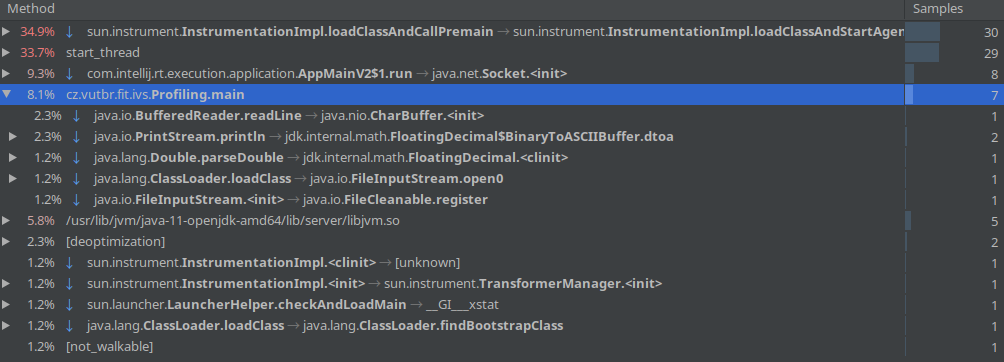
\includegraphics[width=.7\textwidth]{profiling1.png}
	\end{figure}
	
	\begin{figure}[ht]
		\centering
		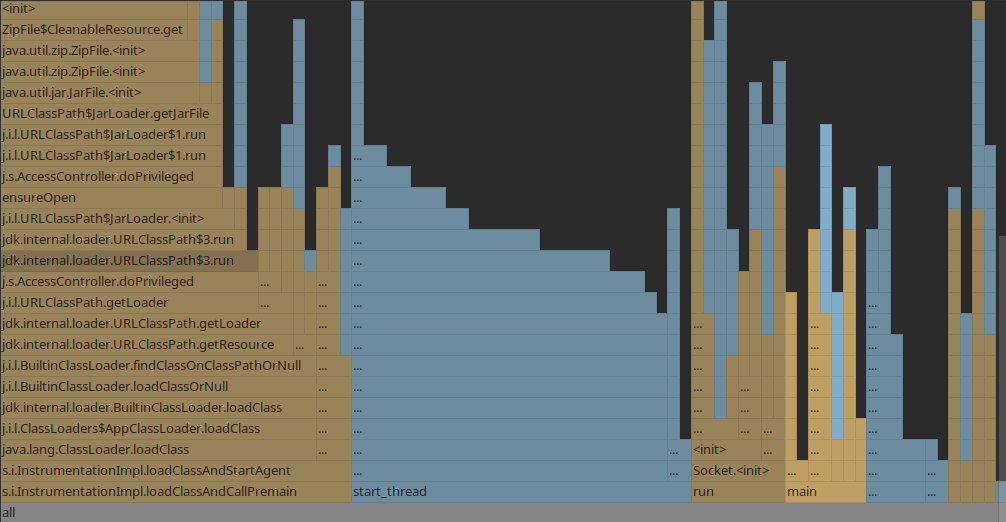
\includegraphics[width=.7\textwidth]{profiling2.png}
	\end{figure}

	\begin{figure}[ht]
		\centering
		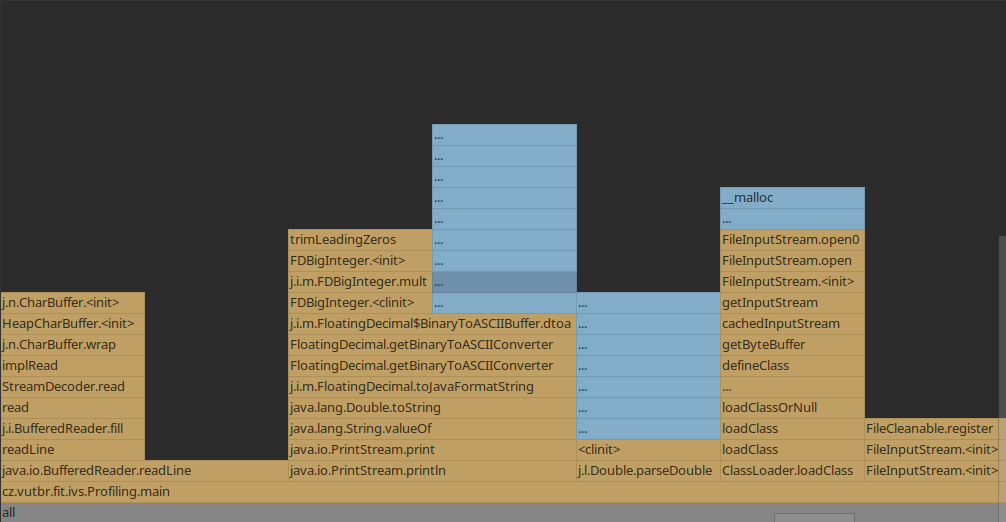
\includegraphics[width=.7\textwidth]{profiling3.png}
	\end{figure}
	
\end{document}